% Drawing 154/09-13 -- folder 154, batch 09, archive page 169 (PDF page 170).
% Transcription: deux grands disques en couleur sans texte, variantes l'un de l'autre : bord vert clair (dans le second, une moitié renforcée en vert foncé), pseudo-droites orange, triangles coloriés en jaune le long du bord, sommets au bord marqués d'un point noir ou d'un trait bleu, et des chemins en tirets noirs qui joignent certains coins en coupant les triangles
% Kind: two disks, variants of each other. Method 2 (schematic redraw from the facsimile). Status: partial.
% Notes: Skeleton. Each disk: the light green rim (the left arc of the second thickened in dark green), seven strands from rim to rim, a marked point at eight places of the rim. The black dashed paths that join corners across the triangles are not drawn. The strands are indicative: they are placed from a page view with their ends on the rim, and neither their number nor the order of their crossings is that of the page; the coloured regions are not drawn. To be redrawn from a full-resolution crop. Redrawn 2026-11-12 (issue 128): to check again.
% Coordinates: 1 unit = 1 mm = 1/100 of the crop width (bbox in page fractions: [0.14, 0.125, 0.96, 0.455]).
% Redrawn by Claude (claude-fable-5-2), issue #128, 2026-11-12; not checked by a human; not compiled (no TeX in the session).
% Rights: reproduces part of the work -- behind RENDER_TRANSCRIPTS, never published by itself.
\documentclass[tikz,border=3pt]{standalone}
\usepackage{amsmath,amssymb}
\usetikzlibrary{patterns,arrows.meta}
\tikzset{Or/.style={orange!90!black}, Lg/.style={green!60!black!70}, Dg/.style={green!45!black}, pencil/.style={black!45}, struck/.style={black!35}, mpt/.style={circle,draw,inner sep=1.3pt}, pt/.style={circle,fill,inner sep=0.9pt}, opt/.style={circle,draw,fill=white,inner sep=1.1pt}}
\begin{document}
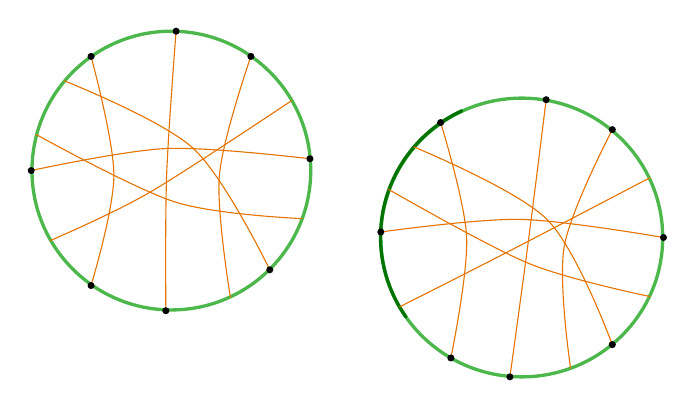
\begin{tikzpicture}[x=1mm,y=1mm,line cap=round,line join=round,font=\scriptsize]
\draw[Lg,very thick] (29.8,-25.3) circle[radius=17.7];
\draw[Lg,very thick] (74.3,-33.8) ellipse[x radius=17.9, y radius=17.7];
\draw[Dg,very thick] (66.7,-17.7) arc[start angle=115, end angle=215, x radius=17.9, y radius=17.7];
\draw[Or] plot[smooth, tension=0.55] coordinates {(30.4,-7.6) (29.2,-25.9) (29.1,-43.1)};
\draw[Or] plot[smooth, tension=0.55] coordinates {(39.9,-10.8) (35.9,-25.9) (37.3,-41.4)};
\draw[Or] plot[smooth, tension=0.55] coordinates {(19.6,-10.8) (22.5,-25.9) (19.6,-39.9)};
\draw[Or] plot[smooth, tension=0.55] coordinates {(12,-25.3) (29.2,-22.5) (47.4,-23.8)};
\draw[Or] plot[smooth, tension=0.55] coordinates {(12.6,-20.7) (30.3,-29.3) (46.4,-31.4)};
\draw[Or] plot[smooth, tension=0.55] coordinates {(16.2,-13.9) (32.6,-22.5) (42.3,-37.9)};
\draw[Or] plot[smooth, tension=0.55] coordinates {(14.4,-34.2) (27,-28.1) (45.1,-16.4)};
\draw[Or] plot[smooth, tension=0.55] coordinates {(77.4,-16.3) (75.2,-33.8) (72.8,-51.5)};
\draw[Or] plot[smooth, tension=0.55] coordinates {(85.8,-20.1) (79.7,-34.9) (80.5,-50.4)};
\draw[Or] plot[smooth, tension=0.55] coordinates {(64,-19.2) (67.3,-33.8) (65.3,-49.1)};
\draw[Or] plot[smooth, tension=0.55] coordinates {(56.4,-33.1) (74.1,-31.5) (92.3,-33.8)};
\draw[Or] plot[smooth, tension=0.55] coordinates {(57.4,-27.7) (75.2,-37.1) (90.6,-41.3)};
\draw[Or] plot[smooth, tension=0.55] coordinates {(60.6,-22.3) (77.5,-31.5) (85.8,-47.4)};
\draw[Or] plot[smooth, tension=0.55] coordinates {(58.8,-42.6) (71.8,-36) (90.6,-26.2)};
\node[pt] at (30.4,-7.6) {};
\node[pt] at (39.9,-10.8) {};
\node[pt] at (47.4,-23.8) {};
\node[pt] at (42.3,-37.9) {};
\node[pt] at (29.1,-43.1) {};
\node[pt] at (19.6,-39.9) {};
\node[pt] at (12,-25.3) {};
\node[pt] at (19.6,-10.8) {};
\node[pt] at (77.4,-16.3) {};
\node[pt] at (85.8,-20.1) {};
\node[pt] at (92.3,-33.8) {};
\node[pt] at (85.8,-47.4) {};
\node[pt] at (72.8,-51.5) {};
\node[pt] at (65.3,-49.1) {};
\node[pt] at (56.4,-33.1) {};
\node[pt] at (64,-19.2) {};
\end{tikzpicture}
\end{document}
